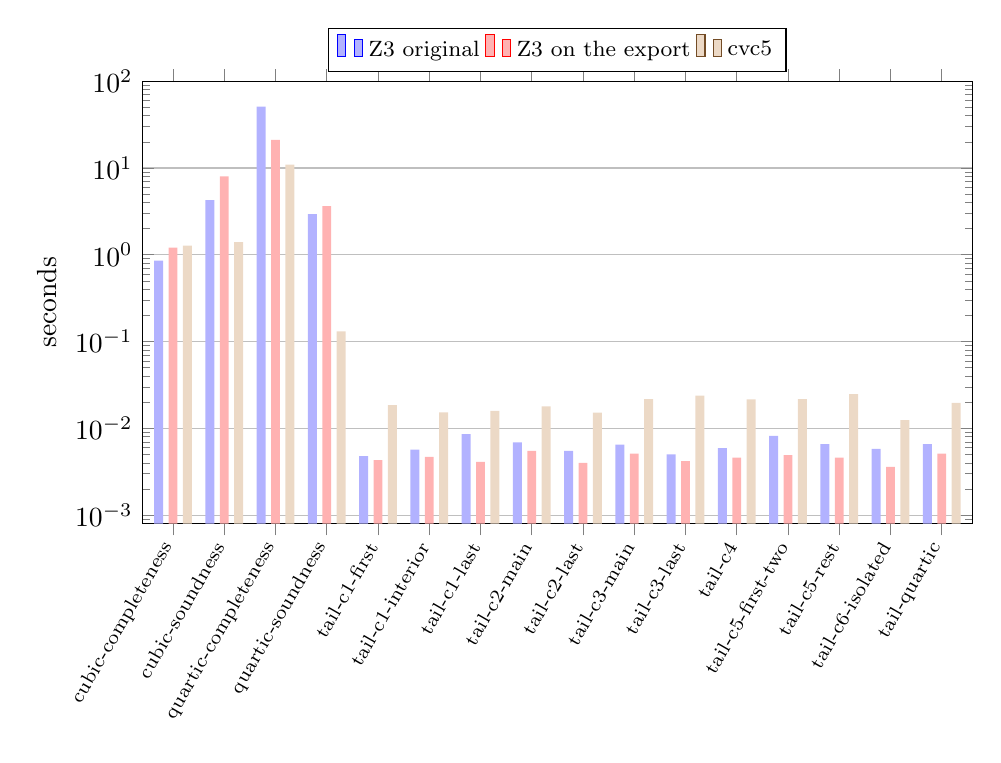
\begin{tikzpicture}\begin{axis}[ybar, width=\linewidth, height=7.2cm, symbolic x coords={cubic-completeness,cubic-soundness,quartic-completeness,quartic-soundness,tail-c1-first,tail-c1-interior,tail-c1-last,tail-c2-main,tail-c2-last,tail-c3-main,tail-c3-last,tail-c4,tail-c5-first-two,tail-c5-rest,tail-c6-isolated,tail-quartic}, xtick=data, x tick label style={rotate=60,anchor=east,font=\scriptsize}, ymode=log, log origin=infty, ymin=0.0008, ymax=100, bar width=3.2pt, enlarge x limits=0.04, ylabel={seconds}, ymajorgrids, legend style={at={(0.5,1.02)},anchor=south,legend columns=3,font=\footnotesize}]
\addplot+[draw=none] coordinates {(cubic-completeness,0.8546) (cubic-soundness,4.2486) (quartic-completeness,51.0015) (quartic-soundness,2.9353) (tail-c1-first,0.0048) (tail-c1-interior,0.0057) (tail-c1-last,0.0086) (tail-c2-main,0.0069) (tail-c2-last,0.0055) (tail-c3-main,0.0065) (tail-c3-last,0.0050) (tail-c4,0.0059) (tail-c5-first-two,0.0082) (tail-c5-rest,0.0066) (tail-c6-isolated,0.0058) (tail-quartic,0.0066)};
\addplot+[draw=none] coordinates {(cubic-completeness,1.2091) (cubic-soundness,8.0113) (quartic-completeness,21.0396) (quartic-soundness,3.6269) (tail-c1-first,0.0043) (tail-c1-interior,0.0047) (tail-c1-last,0.0041) (tail-c2-main,0.0055) (tail-c2-last,0.0040) (tail-c3-main,0.0051) (tail-c3-last,0.0042) (tail-c4,0.0046) (tail-c5-first-two,0.0049) (tail-c5-rest,0.0046) (tail-c6-isolated,0.0036) (tail-quartic,0.0051)};
\addplot+[draw=none] coordinates {(cubic-completeness,1.2736) (cubic-soundness,1.3954) (quartic-completeness,10.9495) (quartic-soundness,0.1312) (tail-c1-first,0.0185) (tail-c1-interior,0.0153) (tail-c1-last,0.0159) (tail-c2-main,0.0179) (tail-c2-last,0.0152) (tail-c3-main,0.0217) (tail-c3-last,0.0239) (tail-c4,0.0215) (tail-c5-first-two,0.0217) (tail-c5-rest,0.0248) (tail-c6-isolated,0.0124) (tail-quartic,0.0196)};
\legend{Z3 original, Z3 on the export, cvc5}\end{axis}\end{tikzpicture}
